\documentclass{resume} % Use the custom resume.cls style

\usepackage[left=0.6in,top=0.8in,right=0.6in,bottom=0.8in]{geometry} % Document margins
\usepackage{xcolor}
\usepackage{hyperref}
\hypersetup{
    colorlinks=true,
    linkcolor=blue,
    filecolor=magenta,      
    urlcolor=teal,
}
\usepackage{graphicx}
\usepackage{enumitem}
\newcommand{\tab}[1]{\hspace{.2667\textwidth}\rlap{#1}}
\newcommand{\itab}[1]{\hspace{0em}\rlap{#1}}
\newcommand{\spazio}{\begin{center} \par\noindent\rule{0.2\textwidth}{0.4pt} \end{center}}

\name{Emilio Berti} % Your name
% \address{
%     \centering
%     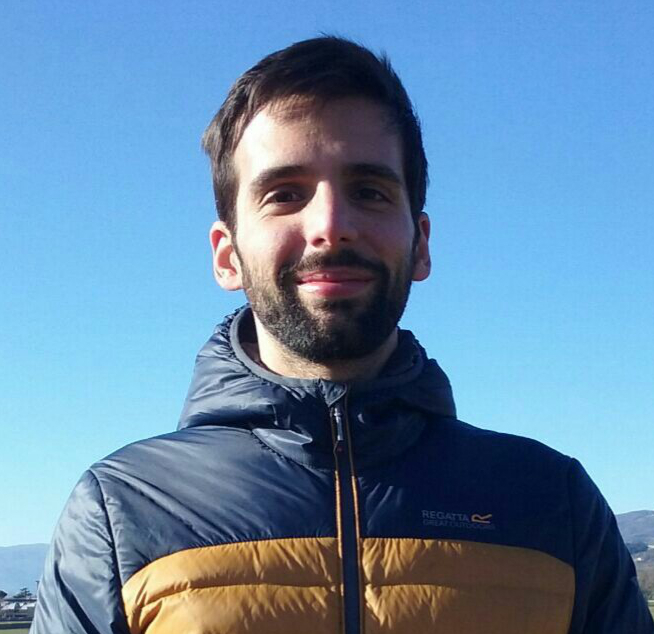
\includegraphics[width=0.30\textwidth]{Emilio.jpg}
% }
\address{(+45) 266 54 662 \\ emilio.berti90@gmail.com \\ \href{https://orcid.org/0000-0001-9286-011X}{ORCID} \\ \href{https://scholar.google.com/citations?user=5KPh-oUAAAAJ&hl=en}{Google scholar} \\ \href{https://emilio-berti.github.io/}{website}}

\begin{document}

\begin{rSection}{Summary}
I am a theoretical ecologist with a passion for math and computing.
I have a strong quantitative background, with expertise in mathematical and statistical modelling of complex systems using big databases at large spatio-temporal scales.
I have worked in many different fields of biology, from molecular muscle physiology to macroecology and biogeography.
I am very open minded to other cultures and societies: I am Italian, my wife is Bulgarian, we met in Denmark, and we live in Germany.
I am an avid reader of ancient history and I love sumo.
\end{rSection}

\begin{rSection}{Professional Experience}
{\bf PostDoctoral researcher} \hfill {\em 01/10/2020 -- Present}\\
Theory in Biodiversity Science, German Centre for Integrative Biodiversity Research (iDiv), Leipzig, Germany

{\bf Scientific consultant} \hfill {\em 01/05/2020 -- 31/07/2020}\\
Department of Bioscience, Aarhus University, Aarhus, Denmark

{\bf Teaching assistant} \hfill {\em 01/02/2017 -- 30/04/2020}\\
Department of Biology, Aarhus University, Aarhus, Denmark

{\bf Internship} \hfill {\em 15/07/2015 -- 16/10/2015}\\
Department of Biology, Florence University, Florence, Italy
\end{rSection}

\begin{rSection}{Education}
{\bf PhD} \hfill {\em 01/02/2017 -- 29/06/2020} 
\\ Section of Ecoinformatics and Biodiversity, Department of Biology, Aarhus University, Aarhus, Denmark.
\\ Title of dissertation: \textit{Megafauna extinctions, allometric scaling and biotic interactions: ecological effects and restoration opportunities through rewilding}.

{\bf Visiting PhD student} \hfill {\em 15/09/2018 -- 12/12/2018}
\\ Department of Ecology and Evolution, University of Chicago, Chicago, IL

{\bf MSc in Biology} \hfill {\em 01/09/2013 -- 31/04/2016}
\\ Department of Ecology and Evolution, University of Florence, Florence, Italy
\\ Title of dissertation: \textit{Analysis of the movement and aggressive interactions between two species of ants of the Genus Lasius (Hymenoptera: Formicidae) through mathematical models}.

{\bf BSc in Biology} \hfill {\em 01/09/2009 -- 31/09/2012}
\\ Department of Physiology, University of Florence, Florence, Italy
\\ Title of dissertation: \textit{The effects of myopalladin on the contraction mechanics of muscle fibers}.
\end{rSection}

\begin{rSection}{Skills}
I have developed an outstanding mathematical and theoretical skill set and successfully applied it to investigate macroecological and biogeographical drivers of biodiversity.
I also have experience with lab and field work, especially on surveys of Mediterranean plants and animals.

{\bf Languages} Italian (native), English (fluent), German (A1), French (A1)\\
{\bf Programming} R, python, bash, C/C++, Stan, javascript (mostly for Google Earth Engine), SQL (postgis flavor), GIS, High Performance Computing (HPC)\\
{\bf Software} Linux/GNU, QGIS, Anaconda, RShiny, Jupyter Notebooks, \LaTeX, Git, GitHub\\
{\bf Methods} 
network theory,
mathematical modeling,
geographic information systems (GIS),
geoinformatics,
geomatics,
biostatistics,
data science,
statistics,
Bayesian inference,
scenario analysis,
trend analysis,
ordination and classification,
optimization,
machine learning,
species distribution models (SDMs),
environmental niche modeling,
community assembly,
climate analyses,
automation.\\
{\bf Relevant courses} Plant biodiversity (focused on Mediterranean ecosystems; MSc), Ecophysiology and climate changes (MSc), Applied plant physiology (MSc), Statistics for experimental research (MSc), Mixed models (PhD).\\
{\bf Relevant lab courses} Inorganic chemistry (BSc), Experimental physics (BSc), GIS for marine biology (MSc).
\end{rSection}

\clearpage

\begin{rSection}{Conference talks as presenter}
\begin{enumerate}[leftmargin=0pt]
    \setcounter{enumi}{0}
    \itemsep-1ex
    \item{Bauer, B., \textbf{Berti, E.}, \dots, \& Brose, U. (2022). From regional to local scale: biotic interactions shape multilayer food-webs. \textit{SFE-GFO-EEF biannual meeting, Metz, France}. \underline{Invited talk}}
    \item{\textbf{Berti, E.}, \& Svenning, J.C. (2022). State-space models show that functional replacements of extinct megafauna have distinct habitat preference in a European rewilding area. \textit{SFE-GFO-EEF biannual meeting, Metz, France}}
    \item{Grenié, M., \textbf{Berti, E.}, Carvajal-Quintero, J., Winter, M., \& Sagouis (2021). Matching Species Names Across Biodiversity Databases: Sources, tools, pitfalls and best practices for taxonomic harmonization. \textit{TDWG annual meeting, online}}
    \item{\textbf{Berti, E.} \& Svenning, J.C. (2019). Megalinkers extinction and the decrease of ecosystem connectivity. \textit{ESA annual meeting, Louisville, KY}}
    \item{\textbf{Berti, E.}, Jarvie, S. W., \& Svenning, J.C. (2018). Rewiring food webs via trophic rewilding. \textit{BES annual meeting, Belfast, UK}}
\end{enumerate}
\end{rSection}

\begin{rSection}{Peer review}
As of February 2024, I have reviewed 7 papers for: Ecography (2), Ecology Letters (2), GigaScience (1), Scientia Agricola (1), and Methods in Ecology and Evolution (1). You can find more at my \href{https://www.webofscience.com/wos/author/record/2190178}{WoS profile}.
\end{rSection}

\begin{rSection}{Supervision and Mentoring}
I am formally co-supervising the PhD candidate Jingyi Li, who is developing a novel mathematical approach for functional responses based on information theory. 
In addition, I provide theoretical, computational, and statistical advice to several members of the TiBS working group at iDiv as well as individual mentoring for PhD students, advising especially on transferable skills and alternative career paths outside academia.
\end{rSection}

\begin{rSection}{Teaching \& Organized Workshops}
During my PhD, I taught one course every semester, as part of my salary was paid by Aarhus University on the basis of teaching.
% I have thus a relatively long teaching experience for my career stage.
In addition, I have regularly organized workshops to teach reproducible research and open data principles and have organized a weekly journal club during my PhD and currently during my PostDoc.

% \spazio
\begin{itemize}
\setlength\itemsep{-0.5em}
    \item Theoretical Population Ecology (2023) -- Teaching assistant (MSc course).
    \item Introduction to scientific programming and tidyverse (2022) (\href{https://emilio-berti.github.io/teaching/tidyverse.html#(1)}{slides}) -- Lecturer (PhD course).
    \item Introduction to git and GitHub for a fool-proof programming (2022) (\href{https://emilio-berti.github.io/idiv-git-introduction/}{course}) -- Lecturer (PhD course).
    \item Meta-analyses for Biodiversity (2021) -- Teaching assistant (MSc course).
    \item Statistical and Geospatial Modelling (2019) -- Teaching assistant (MSc course).
    \item Behavioural Biology (2018, 2019) -- Teaching assistant (BSc course).
    \item Geographic Information System (2017) -- Lab assistant (BSc course).
    \item Cleaning online repository data for use in biogeography and macroecology (2019). -- Co-organizer (Workshop).
    \item Running a species distribution model in R (2019) -- Co-organizer (Workshop).
    \item A (very) gentle introduction to Linux (2019) -- Organizer (Workshop).
\end{itemize}
\end{rSection}

\begin{rSection}{Collaborations}
I have moved several times to pursue my career dreams and, being a friendly person, I established personal and professional ties with the people I met.
My network of current collaborators include:
\begin{itemize}
\setlength\itemsep{-0.5em}
    \item Prof. Jens-Christian Svenning, Aarhus University, Aarhus, Denmark.
    \item Prof. Ulrich Brose, Jena University, Jena, Germany.
    \item Prof. Daniel Reuman, Kansas University, Lawrence, KS, USA.
    \item Prof. Giacomo Santini, Universit\`{a} degli Studi di Firenze, Florence, Italy.
    \item Prof. Kai Yue, Fujian Normal University, Fuzhou, China.
    \item Prof. Neil Carter, University of Michigan, Ann Arbor, MI, USA.
    \item Ass. Prof. Susanne Vogel, Open University of the Netherlands, Heerlen, Netherlands.
    \item Prof. Fritz Vollrath, University of Oxford, Oxford, UK.
\end{itemize}
\end{rSection}

\clearpage
\begin{rSection}{Scientific Publications}

{\underline{First authorship}}
\begin{enumerate}[leftmargin=0pt]
    \itemsep-1ex
    \item{\textbf{Berti, E.}, Rosenbaum, B., Brose, U., \& Vollrath, F. (2023). Energy landscapes direct the movement preferences of elephants. Under review in \textit{Journal of Animal Ecology}. \url{https://doi.org/10.22541/au.168373276.62196439/v1}}
    \item{Bauer, B., \textbf{Berti, E.}, ... \& Brose, U. (2022). Biotic filtering by species’ interactions constrains food-web variability across spatial and abiotic gradients. \textit{Ecology letters}.\url{https://doi.org/10.1111/ele.13995}. (\texttt{Shared first authorship})}
    \item{\textbf{Berti, E.}, Davoli, M., ... \& Vollrath, F. (2021). The r package enerscape: A general energy landscape framework for terrestrial movement ecology. \textit{Methods in Ecology and Evolution}. \url{https://doi.org/10.1111/2041-210X.13734}}
    \item{\textbf{Berti, E.}, Monsarrat, S., Munk, M., Jarvie, S. \& Svenning, J.C. (2020). Body size is a good proxy for vertebrate charisma. \textit{Biological Conservation}. \url{https://doi.org/10.1016/j.biocon.2020.108790}}
    \item{\textbf{Berti, E.} \& Svenning, J.C. (2020). Megafauna extinctions have reduced biotic connectivity worldwide. \textit{Global Ecology and Biogeography}. \url{https://doi.org/10.1111/geb.13182}}
\end{enumerate}
{\underline{Last authorship}}
\begin{enumerate}[leftmargin=0pt]
    \setcounter{enumi}{5}
    \itemsep-1ex
    \item{Gauzens, B., Brose, U., Delmas, E., \& \textbf{Berti, E}. (2023). ATNr: Allometric Trophic Network models in R. \textit{Methods in Ecology and Evolution}. \url{https://doi.org/10.1111/2041-210X.14212}}
\end{enumerate}
{\underline{Co-authorship with supporting role}}
\begin{enumerate}[leftmargin=0pt]
    \setcounter{enumi}{6}
    \itemsep-1ex
    \item Antunes, A. C., \textbf{Berti, E.}, ... \& Gauzens, B. (2023). Linking biodiversity and nature’s contributions to people (NCP): a macroecological energy flux perspective. \textit{Trends in Ecology and Evolution}. \url{https://doi.org/10.1016/j.tree.2024.01.004}
    \item Wei, S., \textbf{Berti, E.}, ... \& Yue, K. (2023). Global patterns and drivers of lead concentration in inland waters. \textit{Journal of Hazardous Materials}. \url{https://doi.org/10.1016/j.jhazmat.2023.132455}
    \item Amyntas, A., \textbf{Berti, E.}, ... \& Brose, U. (2023). Niche complementarity among plants and animals can alter the biodiversity–ecosystem functioning relationship. \textit{Functional Ecology}. \url{https://doi.org/10.1111/1365-2435.14419}
    \item Dyer, A., Brose, U., \textbf{Berti, E.}, Rosenbaum, B., \& Hirt, M. R. (2023). The travel speeds of large animals are limited by their heat-dissipation capacities. \textit{Plos Biology}. \url{https://doi.org/10.1371/journal.pbio.3001820}
    \item Vogel, S. M., ..., \textbf{Berti, E.}, ... \& Svenning, J. C. (2023). Identifying sustainable coexistence potential by integrating willingness-to-coexist with habitat suitability assessments. \textit{Biological Conservation}. \url{https://doi.org/10.1016/j.biocon.2023.109935}
    \item Grenié, M, \textbf{Berti, E.}, ... \& Marten, W. (2022). Harmonizing taxon names in biodiversity data: a review of tools, databases, and best practices. \textit{Methods in Ecology and Evolution}. \url{https://doi.org/10.1111/2041-210X.13802}
    % \item{Terlau, J., ..., \textbf{Berti, E.}, ... \& Hirt, M. R. (2022). Integrating trait-based movement into mechanistic predictions of thermal performance. \textit{Preprint}. \url{http://dx.doi.org/10.21203/rs.3.rs-1815379/v1}}
\end{enumerate}
\end{rSection}

% \begin{rSection}{External Links}
% \begin{minipage}{0.5\textwidth}
% \begin{itemize}
%     \item \href{https://scholar.google.com/citations?user=5KPh-oUAAAAJ&hl=en}{Google Scholar profile}
%     \item \href{https://emilio-berti.github.io/}{Personal website}
%     \item \href{https://orcid.org/0000-0001-9286-011X}{ORCiD}
% \end{itemize}
% \end{minipage}
% \begin{minipage}{0.5\textwidth}
% \begin{itemize}
%     \item \href{https://www.linkedin.com/in/emilio-berti-55a348146}{LinkedIn}
%     \item \href{https://github.com/emilio-berti}{GitHub}
%     \item \href{https://publons.com/wos-op/researcher/4208953/emilio-berti/peer-review/}{Publons}
% \end{itemize}
% \end{minipage}
% \end{rSection}

\end{document}
